\documentclass[conference]{IEEEtran}

\usepackage{booktabs}
\usepackage{graphicx}
\usepackage{multirow}
\usepackage{url}
\usepackage{xcolor}
\usepackage{amsmath}
\usepackage{array}

\graphicspath{{../outputs/paper_figures/}}

\title{AIOpsStressBench: An Offline Stress-to-Decision Benchmark for Operational Time-Series Forecasting}

\author{
\IEEEauthorblockN{Anonymous Authors}
\IEEEauthorblockA{Anonymous Affiliation}
}

\begin{document}
\maketitle

\begin{abstract}
Time-series forecasting is widely used in cloud operations for capacity planning, alerting, and risk mitigation, but standard benchmarks usually evaluate models on clean, synchronized, offline data. Operational telemetry can be missing, delayed, partially unavailable, shifted by workload changes, and constrained by latency and memory budgets. We present AIOpsStressBench, a reproducible offline stress-to-decision benchmark for operational time-series forecasting. It combines public CloudOps/AIOps telemetry, controlled telemetry-stress operators, latency and memory profiling, severity analysis, and a forecast-to-capacity decision proxy. Rather than asking only which model minimizes clean MSE, the benchmark tests whether model rankings remain stable when telemetry health, latency budgets, and asymmetric decision costs change. Across two multivariate operational traces, we find that the clean-MSE winner, the lowest-latency learned model, and the lowest decision-cost model often differ. Patch-based context modeling improves robustness under metric-channel outage, but this advantage is stress-family specific and incurs higher inference cost. AIOpsStressBench is intended as a complementary evaluation layer for operational forecasting, not as an autoscaling system or a replacement for clean forecasting benchmarks.
\end{abstract}

\begin{IEEEkeywords}
AIOps, time-series forecasting, deployment stress, robustness, latency, CloudOps
\end{IEEEkeywords}

\section{Introduction}

Cloud operations increasingly rely on time-series forecasting to support resource planning, autoscaling, alerting, and operational risk control. Forecasts of CPU utilization, memory pressure, network traffic, disk IO, and operational KPIs can determine whether a system scales early enough before a workload spike, avoids unnecessary over-provisioning, or detects abnormal behavior before users are affected. In this setting, forecasting errors have direct operational meaning: underestimation can translate into resource starvation and risk, while overestimation can lead to persistent waste.

Most long-term time-series forecasting studies evaluate models under a clean offline protocol, even when they introduce stronger backbones such as linear decomposition, patch-based Transformers, inverted attention, or multiscale mixing \cite{dlinear,patchtst,itransformer,timemixer}. The input window is assumed to be available, synchronized, and drawn from a stable distribution. This assumption is too optimistic for CloudOps telemetry. Monitoring pipelines can drop individual points, lose entire metric channels, delay recent samples, or observe sudden level shifts after releases, migrations, workload changes, and mitigation actions. At the same time, online forecasting can be constrained by P95 latency, memory footprint, and update cost.

This paper studies AIOps forecasting under controlled offline deployment-stress. We build AIOpsStressBench, a reproducible evaluation pipeline that combines public operational datasets, stress protocols, deployment-cost metrics, a forecast-to-capacity decision proxy, and case studies. The core question is not which model wins a clean leaderboard, but whether clean-model rankings remain stable when telemetry health, latency budget, and asymmetric decision costs change. Thus AIOpsStressBench is a stress-to-decision benchmark for within-protocol model-selection evidence on public operational telemetry.

The paper is not a method-first forecasting paper and does not claim a new forecasting architecture. RACE-DLinear is included only as a lightweight robust baseline. The contribution is the benchmark protocol and the resulting accuracy--robustness--latency--decision analysis.

Our contributions are:
\begin{itemize}
    \item We introduce AIOpsStressBench, a reproducible offline benchmark artifact for operational forecasting that combines public telemetry traces, fixed chronological splits, controlled telemetry-stress operators, and table/figure generation scripts.
    \item We define a stress-to-decision evaluation protocol that jointly reports forecast accuracy, stress robustness, P95 latency, memory, and a forecast-to-capacity decision proxy.
    \item We provide cross-source model-selection evidence showing that the clean-MSE winner, the lowest-latency learned model, and the lowest decision-cost model can differ under the same operational telemetry protocol.
    \item We document boundary conditions for the benchmark, including synthetic stress realism, KPI-versus-resource dataset roles, reactive-controller references, bounded foundation-model evidence, and reproducibility requirements.
\end{itemize}

\section{Related Work}

\noindent\textbf{Long-term forecasting backbones and benchmarks.}
Recent long-term forecasting work has improved accuracy through simple decomposition, patch tokenization, channel-wise inversion, multiscale mixing, and temporal variation modeling \cite{dlinear,patchtst,itransformer,timemixer,timesnet}. Forecasting benchmarks and archives such as M4, Monash, GIFT-Eval, and fev-bench broaden empirical comparison, reproducible infrastructure, covariate coverage, and aggregation rigor across domains and models \cite{m4,monash,gifteval,fevbench}. These efforts are important context, but their standard clean-data protocols do not directly answer whether a model remains deployable when telemetry is missing, delayed, shifted, or latency constrained.

\noindent\textbf{Foundation models for time series.}
Foundation models such as Chronos, Moirai, and TimesFM study pretraining and zero-shot forecasting across diverse time-series corpora \cite{chronos,moirai,timesfm}. Recent efficiency studies further argue that time-series foundation models should be evaluated with runtime or energy cost, not only accuracy \cite{fmenergy}. They are relevant to CloudOps because operational telemetry can be heterogeneous and costly to label or tune. This paper does not claim a systematic foundation-model benchmark. We include only a bounded Chronos-Bolt zero-shot reference on the two multivariate sources to report feasibility, latency, and stress sensitivity, while the main empirical claims remain restricted to reproducible supervised and official backbone comparisons under the native stress protocol.

\noindent\textbf{AIOps telemetry, autoscaling, and public traces.}
CloudOps forecasting has recently received more attention through large-scale pretraining datasets such as the Salesforce CloudOps collection \cite{cloudops}. Observability-native benchmarks such as BOOM show that production observability metrics have heavy-tailed, heterogeneous structure and deserve domain-specific evaluation \cite{boom}. Public AIOps and cluster traces also support reproducible operational studies, including GAIA \cite{gaia}, NetMan KPI datasets \cite{netman}, Alibaba Cluster Trace 2018 \cite{alibaba}, and Borg-style workload traces inside the Salesforce CloudOps release. Autoscaling and resource-management systems such as Autopilot, Sinan, and AHPA motivate why forecast quality should be connected to operational cost and resource risk \cite{autopilot,sinan,ahpa}. Monitoring systems also expose practical telemetry concerns: missing data handling, metric freshness, stale series, and unavailable pod metrics are explicit operational cases in production monitoring and autoscaling documentation \cite{gcm_missing,gcm_latency,prom_staleness,k8s_hpa}. These sources and systems differ in granularity and application meaning; GAIA and NetMan are strong for KPI stress diversity, while Alibaba and Salesforce/Borg better support multivariate operational telemetry analysis.

\noindent\textbf{Robust and deployment-aware evaluation.}
Missing-value models and imputation methods such as GRU-D and BRITS show that incomplete time series need explicit treatment \cite{grud,brits}. Drift and out-of-distribution studies further show that clean validation can fail when the test distribution changes \cite{onenet,woods}. Robustness benchmarks such as WOODS study distribution shift, while observability benchmarks such as BOOM characterize production telemetry structure. AIOpsStressBench targets the gap between these lines: it does not compete on archive scale, but couples public operational telemetry, controlled telemetry-degradation operators, latency/memory profiling, a forecast-to-capacity decision proxy, and model-selection analysis in one reproducible stress-to-decision protocol.

Existing clean forecasting, robustness, observability, and foundation-model benchmarks answer important but different questions. AIOpsStressBench narrows the target to a joint stress-to-decision question: under the same public operational trace, do telemetry degradation, latency budget, and asymmetric decision cost change which forecaster a practitioner would select?

\section{Application Scenario}

We consider a cloud platform where machines, services, or KPI streams emit telemetry such as CPU utilization, memory utilization, network traffic, disk IO, and operational KPI values. A forecasting service receives the recent telemetry window and predicts a future horizon used by capacity planning, alerting, or autoscaling decisions.

The deployment setting differs from clean forecasting benchmarks in four ways. First, monitoring systems can drop individual samples or entire metrics. Second, recent telemetry can arrive late, making the tail of the context window unreliable. Third, workload bursts and operational changes can shift the recent context. Fourth, online inference may be constrained by latency and memory budgets. These constraints motivate an Applied evaluation that reports robustness and deployment cost, not only MSE and MAE.

We separate three deployment paths. A low-latency alerting path needs a cheap forecast every few minutes and should prioritize P95 latency and predictable memory use. A batch capacity-planning path can spend more compute but must reduce under-provisioning and peak misses over a longer horizon. A degraded-telemetry response path must remain meaningful when telemetry itself is unreliable, for example when a monitoring exporter stops reporting a metric channel. A single clean MSE table cannot distinguish these paths, so our evaluation asks which model is appropriate for each operational constraint.

\section{Evaluation Pipeline}

The evaluation pipeline has six stages. First, each dataset is audited and converted to a tensor with shape $[\text{entities}, \text{time}, \text{metrics}]$. Second, a rolling-window forecasting task is built with input length 96 and prediction horizon 24. Third, deployment stress is injected into the input window. Fourth, each model is evaluated by forecasting accuracy, latency, memory, and parameters. Fifth, predictions are passed to a forecast-to-capacity decision proxy. Sixth, selected windows are visualized as case studies.

\begin{figure}[t]
\centering
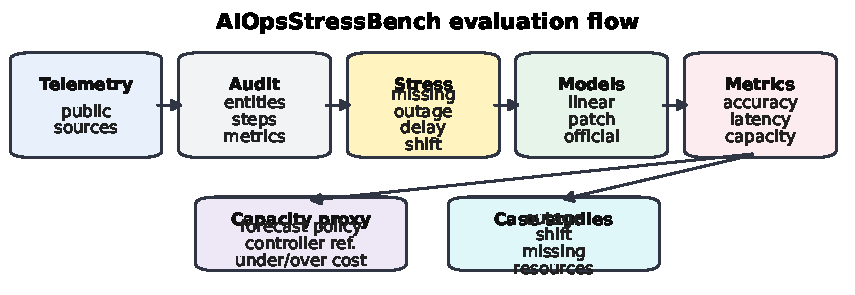
\includegraphics[width=\linewidth]{figure_aiopsstressbench_pipeline.pdf}
\caption{AIOpsStressBench pipeline. Public telemetry is audited, windowed, evaluated under controlled offline deployment-stress operators, profiled for latency and memory, and connected to within-protocol decision-proxy analysis and case studies.}
\label{fig:pipeline}
\end{figure}

\begin{table}[t]
\centering
\tiny
\caption{AIOpsStressBench benchmark card.}
\label{tab:benchmark-card}
\resizebox{\columnwidth}{!}{%
\begin{tabular}{p{0.18\linewidth}p{0.32\linewidth}p{0.39\linewidth}}
\toprule
Component & Setting & Details \\
\midrule
Task & Operational forecasting under deployment stress & Input length 96, horizon 24, chronological 65/15/20 split. \\
Public sources & GAIA, NetMan, Alibaba 2018, Salesforce/Borg 2011 & Alibaba and Salesforce/Borg are multivariate telemetry; GAIA/NetMan provide KPI stress diversity. \\
Stress operators & Missing points, metric outage, delayed tail, noise, burst, level shift & Stress is injected only into the input window; targets remain clean. \\
Metrics & MSE/MAE plus deployment metrics & P95 latency, parameters, memory, severity slope, and forecast-to-capacity proxy. \\
Core comparable pool & DLinear, RACE-DLinear, PatchTST-lite, official PatchTST, native iTransformer, TimeMixer & Native or native-wrapper stress protocol where available; RACE-DLinear is a lightweight stress-aware baseline used for robustness analysis. \\
Reference-only pool & LastValue, Chronos-Bolt zero-shot, LTSF-bridge iTransformer & Context, lower-bound, and feasibility references; these rows do not drive the central model-ranking claims. \\
Reproducibility & Minimal and extended reproduction paths & Minimal path regenerates the core winner and latency tables; extended path regenerates severity, sensitivity, and multi-seed results. \\
\bottomrule
\end{tabular}
}
\end{table}


\subsection{Deployment Stress Protocol}

All experiments use input length 96, prediction horizon 24, seed 42, and chronological train/validation/test splits of 65\%/15\%/20\%. Stress is applied only to the input window at train or evaluation time; the forecasting target remains clean, so the protocol measures whether a model can make an operationally useful forecast from degraded telemetry.

We evaluate six deployment stresses. Missing points randomly mask individual input values. Missing variables mask entire metric channels within an input window, simulating telemetry outage. Delayed tail masks the most recent 12 input steps, simulating late-arriving monitoring data. Noisy stress adds Gaussian input noise with standard deviation 0.2. Burst stress injects sparse positive spikes at rate 0.02. Level shift adds a constant shift of 0.4 to the second half of the input window, simulating release, migration, or workload-regime changes. These stresses are not meant to cover every production failure mode; they provide a reproducible minimum protocol for deployment-aware forecasting.

\begin{table}[t]
\centering
\tiny
\caption{Deployment-stress taxonomy and operational motivation.}
\label{tab:stress-taxonomy}
\resizebox{\columnwidth}{!}{%
\begin{tabular}{p{0.16\linewidth}p{0.28\linewidth}p{0.29\linewidth}p{0.18\linewidth}}
\toprule
Stress & Protocol & Operational source & Evaluation \\
\midrule
Missing points & Random input values unavailable & Packet loss, scraper gaps & Robustness curve \\
Metric outage & Entire input metric channel masked & Exporter failure, telemetry outage & Outage stress \\
Delayed tail & Most recent k input steps hidden & Ingestion lag, delayed monitoring & Delay stress \\
Noise & Gaussian perturbation on input & Aggregation or sensor instability & Noise stress \\
Burst & Sparse positive spikes in input & Workload spike, flash crowd & Burst stress \\
Level shift & Context level changes before horizon & Release, migration, mitigation & Shift stress \\
\bottomrule
\end{tabular}
}
\end{table}


\subsection{Stress Realism Audit}

Public operational traces are often cleaned before release and underrepresent monitoring failures, so we treat stress realism as calibration rather than validation. We audit observable public-trace proxies such as non-finite values, zero rates, long zero runs, flatline windows, robust spikes, and level-shift scores. These proxies motivate stress levels and boundary conditions, but they do not estimate operator-specific incident frequency or uniquely identify root causes such as exporter failure or ingestion delay. Metric outage has the clearest public-trace proxy support in Alibaba and Salesforce/Borg, while point missingness and tail delay remain controlled probes for reproducible sensitivity analysis.

The public RE2-OB fault-injection slice is an external sanity check rather than incident validation. It is evaluated without injected corruption and tests whether naturally induced fault windows can expose the same type of ranking disagreement. Because the target is Istio P99 latency rather than resource demand, its asymmetric proxy is reported as decision cost rather than resource-capacity cost. Table~\ref{tab:public-fault-mini} summarizes the resulting 58 parsed cases.

\begin{table}[t]
\centering
\scriptsize
\caption{External RE2-OB fault-window sanity check. It is not used for resource-capacity claims.}
\label{tab:public-fault-mini}
\resizebox{\columnwidth}{!}{%
\begin{tabular}{llrllrl}
\toprule
Dataset & Slice & Cases & Target & MSE changes & MSE/decision & Role \\
\midrule
RE2-OB & fault injection & 58 & Istio P99 & 9 & 11 & sanity check \\
\bottomrule
\end{tabular}
}
\end{table}


\section{Datasets}

GAIA metric forecast contains operational KPI series with categories such as periodic, changepoint, low-SNR, and partially-stationary behavior. It is useful for stress diversity, but it is mostly single-target KPI data.

NetMan KPI provides another public operational KPI source and supports missing-telemetry case studies. Like GAIA, it should not be overused for resource-capacity claims.

Alibaba Cluster Trace 2018 machine usage is the first multivariate source. We use machine-level CPU utilization, memory utilization, network in/out, and disk IO. It supports a resource-telemetry story, but it should not be described as service-level request telemetry.

Salesforce CloudOps/Borg 2011 is the second multivariate operational source. We convert the public Salesforce CloudOps TSF Borg split into a tensor with 256 entities, 2048 time steps, and 7 dynamic metrics. One caveat is that \texttt{dynamic\_4} is all zero in the current subset; we keep it in the released tensor for source-schema reproducibility and audit transparency, but exclude it from metric-level interpretation. This dataset strengthens the multi-source evidence because the same native stress suite, StressRoute policy, official baselines, severity curves, and multi-seed checks are reproduced beyond Alibaba.

We use the datasets for different evidential roles. GAIA and NetMan support KPI stress diversity and degraded-telemetry case studies. Alibaba and Salesforce/Borg provide the main multivariate resource-telemetry evidence for latency, stress, and capacity-proxy analysis. Capacity-related conclusions are therefore reported only for resource-level telemetry sources and should not be extrapolated from KPI-only datasets.

\section{Baselines}

Native pipeline baselines include last-value, DLinear, RACE-DLinear, and a lightweight patch-based model. We use PatchTST-lite to denote our lightweight native patch-based implementation evaluated inside the unified NPZ/stress pipeline, and Official PatchTST to denote the imported official backbone evaluated through a native wrapper. RACE-DLinear is not the main contribution; it is a lightweight robust baseline used to test whether simple missing-aware linear modeling can improve deployment-stress behavior.

Official PatchTST is integrated by importing the official model class and evaluating it inside the native NPZ/stress pipeline. This keeps missing-variable stress and decision-proxy evaluation comparable with native baselines. Official iTransformer and TimeMixer are evaluated with native wrappers on the two multivariate telemetry sources for the core deployment stresses. Chronos-Bolt is evaluated only as a zero-shot target-metric reference on a bounded subset, not as a full foundation-model benchmark. Older LTSF-bridge iTransformer runs are retained only as reference analysis because they flatten entity-metric channels and are not perfectly equivalent to the native per-entity target protocol.

Baseline comparability is enforced by the native NPZ windows, the same stress operators, the same target metric, and the same latency profiler. The main winner tables exclude LastValue, Chronos-Bolt, and LTSF-bridge rows from learned-model selection; implementation, budget, and coverage details are summarized in the generated baseline-fairness card.

\section{Metrics}

We report MSE and MAE, but they are not sufficient for the Applied story. We also report P95 latency, parameter count, GPU memory, and a forecast-to-capacity decision proxy.

The forecast-to-capacity decision proxy compares predicted capacity with true demand under a headroom factor. It penalizes under-provisioning more heavily than over-provisioning:
\begin{equation}
\text{cost} = c_u \frac{\max(y - \hat{y}(1+h), 0)}{\max(|y|, \epsilon)}
 + c_o \frac{\max(\hat{y}(1+h)-y, 0)}{\max(|y|, \epsilon)}.
\end{equation}
This metric is a decision proxy rather than an autoscaling system. It intentionally excludes queueing, cold starts, scheduler constraints, service dependencies, closed-loop control delay, and service-level SLOs. We use the proxy for one narrow purpose: to test whether forecasts with similar MSE can imply different under- and over-provisioning consequences under a fixed asymmetric-cost protocol. The default $c_u:c_o=5:1$ encodes the operational assumption that resource starvation or missed capacity is more costly than short-lived over-provisioning waste; Table~\ref{tab:capacity-sensitivity-compact} reports compact sensitivity checks.

Unless otherwise noted, we use headroom $h=0.15$, under-provision cost $c_u=5.0$, over-provision cost $c_o=1.0$, and demand floor $\epsilon=0.05$. The target is metric index 0 for each dataset. Costs are computed per entity, window, horizon step, and target metric, then averaged over the evaluated test windows. The same target metric is used for forecast accuracy and the capacity proxy.

\subsection{Forecast-to-Capacity Decision Proxy}

To make the Applied evaluation less dependent on MSE and MAE, we add a forecast-to-capacity decision proxy. A forecast policy provisions $\max(\hat{y},0)(1+h)$ capacity for the future horizon. We compare forecasting policies with LastObserved and Reactive HPA references. LastObserved repeats the latest observed value, while Reactive HPA uses the previous realized demand as a one-step delayed controller sanity reference. The proxy reports under-provision area, over-provision area, peak-miss rate, severe-under rate, P95 under-provision ratio, and total normalized cost. Reactive HPA is not a proactive long-horizon forecasting policy; its latency is reported as a controller reference, and it is not eligible for clean/stress forecasting winner selection.

\section{Results}

We organize the results around three claims. Claim 1 asks whether clean accuracy is sufficient for within-protocol model selection. Claim 2 tests whether robustness depends on the stress family. Claim 3 connects benchmark evidence to deployment constraints such as latency budgets and decision-proxy objectives.

The results are organized as an evidence chain rather than as a raw leaderboard. Claim 1 is anchored by the cross-source winner table, which tests whether clean-MSE, lowest-latency, and decision-cost winners agree on Alibaba and Salesforce/Borg. Claim 2 is supported by stress-family and severity analyses, which test whether robustness is operator-specific. Claim 3 is supported by latency, memory, decision-proxy, and sensitivity tables, which test whether deployment constraints change the selected model. Extended sweeps and auxiliary ablations are part of the reproducibility package.

\begin{table}[t]
\centering
\tiny
\caption{Cross-source scenario winners in the single-run all-model pool. The table tests whether best-MSE, lowest-P95 learned, and best decision-cost models agree under the same source and stress setting. LastValue, Chronos-Bolt, and LTSF-bridge are excluded from winner selection; multi-seed stability is reported in Table~\ref{tab:multiseed-compact}.}
\label{tab:cross-source-winners}
\resizebox{\columnwidth}{!}{%
\begin{tabular}{llllllc}
\toprule
Source & Stress & Pool & Best MSE & Best P95 & Best decision & Flip \\
\midrule
Alibaba & Clean & all learned & RACE-DLinear & DLinear & Native iTransformer & Y \\
Alibaba & Delayed tail & all learned & RACE-DLinear & DLinear & Official PatchTST & Y \\
Alibaba & Missing points & all learned & DLinear & DLinear & Official PatchTST & Y \\
Alibaba & Metric outage & all learned & PatchTST-lite & DLinear & PatchTST-lite & Y \\
Salesforce/Borg & Clean & all learned & Official TimeMixer & Official PatchTST & Official TimeMixer & Y \\
Salesforce/Borg & Delayed tail & all learned & Official TimeMixer & Native iTransformer & Official PatchTST & Y \\
Salesforce/Borg & Missing points & all learned & Official TimeMixer & Native iTransformer & Official PatchTST & Y \\
Salesforce/Borg & Metric outage & all learned & Native iTransformer & Native iTransformer & Native iTransformer & N \\
\bottomrule
\end{tabular}
}
\end{table}


\subsection{Claim 1: Clean Accuracy Is Insufficient}

Takeaway: clean accuracy is necessary for filtering models, but it is insufficient for selecting an operational forecaster under latency and decision-proxy constraints.

Table~\ref{tab:cross-source-winners} is the first result table because it shows the model-selection problem across both multivariate sources. In most compact source-stress settings, the best clean/stressed MSE model, the lowest-P95 learned model, and the lowest decision-cost model are not all the same. Figure~\ref{fig:multisource-stress}(d) uses the same eight compact settings as its denominator. Salesforce/Borg is not only a supporting appendix row: it reproduces the same objective-disagreement pattern under clean, delayed-tail, and missing-point settings, while metric outage selects native iTransformer across all three objectives in the single-run all-model pool. The point is not that one model always wins; it is that the selected model depends on the operational objective.

Table~\ref{tab:clean-alibaba} then gives the detailed Alibaba clean row behind the compact winner summary. RACE-DLinear obtains the lowest clean MSE, but its advantage over DLinear is small. DLinear is slightly less accurate, yet it is the lowest-latency learned model. PatchTST-lite, Official PatchTST, native iTransformer, and official TimeMixer are close in clean accuracy, but they require higher inference cost. The TimeMixer result is useful because it broadens the model pool without changing the deployment conclusion: a stronger modern backbone is not automatically the right online model when latency is a hard constraint.

This result is already a warning for within-protocol model selection. A clean leaderboard would favor the best MSE row, but an online monitoring path with a strict P95 latency budget may reasonably select a faster learned model, while an offline planning job may accept a heavier model if it lowers decision cost. Clean accuracy is therefore a necessary metric, not a sufficient Applied decision rule. The main evidence for this claim is Table~\ref{tab:cross-source-winners}, the Alibaba detail in Table~\ref{tab:clean-alibaba}, and the five-seed stability check in Table~\ref{tab:multiseed-compact}.

\begin{table}[t]
\centering
\scriptsize
\caption{Clean Alibaba forecasting accuracy and deployment cost.}
\label{tab:clean-alibaba}
\resizebox{\columnwidth}{!}{%
\begin{tabular}{lrrrrr}
\toprule
Model & MSE & MAE & P95 ms & Params & Mem MB \\
\midrule
RACE-DLinear & 0.2671 & 0.3783 & 0.355 & 4668.0 & 17.00 \\
DLinear & 0.2697 & 0.3837 & 0.1369 & 2334.0 & 17.00 \\
Native iTransformer & 0.2744 & 0.3744 & 1.9605 & 2.81e+05 & 30.00 \\
Official PatchTST & 0.2748 & 0.3764 & 2.1504 & 3.06e+05 & 155.0 \\
PatchTST-lite & 0.2753 & 0.3845 & 0.6482 & 1.24e+05 & 37.00 \\
Official TimeMixer & 0.277 & 0.3799 & 4.9689 & 1.29e+05 & 178 \\
Chronos-Bolt ref. & 0.3922 & 0.4705 & 10.95 & pretrained & 26.00 \\
LastValue & 0.4082 & 0.4475 & 0.0734 & 0 & 0 \\
\bottomrule
\end{tabular}
}
\end{table}


\subsection{Claim 2: Robustness Is Stress-Family Specific}

Takeaway: robustness is stress-family specific; patch-based context helps most under metric outage, but this advantage does not automatically transfer to every telemetry corruption.

Table~\ref{tab:stress-alibaba} evaluates the same models after deployment stress is injected into the input window. Among native stress-suite models, PatchTST-lite has the best mean stress MSE and worst-case MSE, suggesting that patch-based context modeling can improve robustness under corrupted telemetry. DLinear remains much faster but loses robustness under severe stress. RACE-DLinear slightly improves over DLinear in mean and worst stress MSE, but the margin is not large enough to support a new-model claim.

Official PatchTST, native iTransformer, and official TimeMixer are evaluated on the same Alibaba native stress suite for core deployment stresses. They are competitive on several clean or mild-corruption scenarios but remain heavier than the native lightweight baselines, and metric outage is still difficult. TimeMixer broadens the model pool through multiscale mixing, but the current native run does not remove the need for channel-outage-specific robustness: losing an entire telemetry stream remains different from modeling multi-scale trends. We also include a bounded Chronos-Bolt zero-shot feasibility reference. It is not a core ranking result or a complete foundation-model comparison; the Applied takeaway is that one pretrained reference does not remove the need for deployment-aware model selection.

\begin{table}[t]
\centering
\scriptsize
\caption{Alibaba deployment-stress robustness.}
\label{tab:stress-alibaba}
\resizebox{\columnwidth}{!}{%
\begin{tabular}{lrrrrr}
\toprule
Model & Mean MSE & Mean MAE & Worst MSE & P95 ms & Mem MB \\
\midrule
PatchTST-lite & 0.2981 & 0.4044 & 0.3486 & 0.665 & 37.00 \\
RACE-DLinear & 0.3086 & 0.4151 & 0.4484 & 0.3899 & 17.00 \\
DLinear & 0.3122 & 0.4206 & 0.464 & 0.1439 & 17.00 \\
Official PatchTST & 0.3178 & 0.4086 & 0.5295 & 1.9425 & 155.0 \\
Official TimeMixer & 0.333 & 0.4156 & 0.522 & 4.6647 & 179 \\
Native iTransformer & 0.3407 & 0.4207 & 0.5309 & 1.911 & 30.00 \\
Chronos-Bolt ref. & 0.4827 & 0.5139 & 0.5212 & 11.71 & 26.00 \\
LastValue & 0.6803 & 0.601 & 1.1093 & 0.0737 & 0.1429 \\
\bottomrule
\end{tabular}
}
\end{table}


The same stress-family pattern appears beyond the Alibaba detail table. On metric outage, DLinear degrades faster than PatchTST-lite on both multivariate sources, with a larger absolute slope on Salesforce/Borg. Under additive noise, the degradation slopes of DLinear, RACE-DLinear, and PatchTST-lite are much closer. The evidence for this claim is Table~\ref{tab:stress-alibaba}, Figure~\ref{fig:multisource-stress}, and the five-seed stability check in Table~\ref{tab:multiseed-compact}; the practical implication is that ``robust model'' is not a single global label.

\subsection{Imputation Check: Does Simple Repair Remove the Problem?}

Takeaway: common imputation pipelines can reduce point-missing damage, but they do not eliminate deployment-stress evaluation because channel outage and stale context still change the model choice.

Real monitoring pipelines often apply simple repair before forecasting. We therefore add DLinear and PatchTST-lite with forward-fill and mean-fill preprocessing after stress injection. The ground truth remains clean. Table~\ref{tab:imputation-pipeline} treats these rows as pipeline baselines, not as new forecasting architectures. If simple imputation solves a stress family, the benchmark should show that; if it does not, the remaining gap is stronger evidence that AIOps forecasting must evaluate degraded telemetry explicitly.

\begin{table}[t]
\centering
\tiny
\caption{Compact imputation check. Simple fill helps point missingness but does not repair whole metric-channel outage.}
\label{tab:imputation-pipeline}
\resizebox{\columnwidth}{!}{%
\begin{tabular}{llllrrr}
\toprule
Source & Stress & Model & Preprocess & MSE & Cap. cost & P95 ms \\
\midrule
Alibaba & missing\_30 & DLinear & None & 0.2866 & 0.5081 & 0.6287 \\
Alibaba & missing\_30 & DLinear & Forward fill & 0.274 & 0.4154 & 0.5726 \\
Alibaba & missing\_30 & DLinear & Mean fill & 0.2744 & 0.4141 & 0.2349 \\
Alibaba & missing\_variables\_30 & DLinear & None & 0.4617 & 0.8886 & 0.2441 \\
Alibaba & missing\_variables\_30 & DLinear & Forward fill & 0.4617 & 0.8886 & 0.6966 \\
Alibaba & missing\_variables\_30 & DLinear & Mean fill & 0.4617 & 0.8886 & 0.7001 \\
Salesforce/Borg & missing\_30 & PatchTST-lite & None & 0.0345 & 0.1756 & 1.1839 \\
Salesforce/Borg & missing\_30 & PatchTST-lite & Mean fill & 0.0282 & 0.1666 & 1.1873 \\
Salesforce/Borg & missing\_variables\_30 & PatchTST-lite & None & 0.0901 & 0.2788 & 0.8685 \\
Salesforce/Borg & missing\_variables\_30 & PatchTST-lite & Forward fill & 0.0901 & 0.2788 & 0.9912 \\
\bottomrule
\end{tabular}
}
\end{table}


The pattern is consistent with deployment intuition. On point missingness, simple repair can help: Alibaba DLinear missing-30 capacity cost drops from 0.508 without repair to about 0.414--0.415 with mean or forward-fill. However, whole-channel outage is not solved by filling because the missing channel carries no contemporaneous information in the window; Alibaba DLinear missing-variable capacity cost remains 0.889 across no-fill, forward-fill, and mean-fill. Thus imputation is a useful pipeline baseline, but it does not remove the need to evaluate telemetry outage and stale-context stresses.

\subsection{Claim 3a: Capacity Objectives Change Model Choice}

Takeaway: the forecast-to-capacity decision proxy exposes consequences that are hidden by MSE/MAE alone, especially when under-provisioning and over-provisioning have asymmetric costs.

Table~\ref{tab:deployment-cost} summarizes deployment cost on Alibaba. LastValue is a useful zero-parameter lower bound for latency, but among learned forecasters DLinear is the lowest-cost option. PatchTST-lite increases latency and memory for better stress accuracy, while Official PatchTST, native iTransformer, and official TimeMixer are heavier references. This cost table is important because AIOps-style workflows often contain both low-latency monitoring paths and slower offline planning paths.
GPU memory is measured by the per-run profiler and rounded to MB; 1 MB-level TimeMixer differences across clean, stress, and aggregate rows reflect measurement aggregation variance rather than configuration changes.

\begin{table}[t]
\centering
\scriptsize
\caption{Alibaba deployment cost across clean and stress runs.}
\label{tab:deployment-cost}
\resizebox{\columnwidth}{!}{%
\begin{tabular}{lrrrr}
\toprule
Model & Clean P95 & Mean P95 & Params & Mem MB \\
\midrule
LastValue & 0.0734 & 0.0736 & 0 & 0.125 \\
DLinear & 0.1369 & 0.143 & 2334.0 & 17.00 \\
RACE-DLinear & 0.355 & 0.3855 & 4668.0 & 17.00 \\
PatchTST-lite & 0.6482 & 0.6629 & 1.24e+05 & 37.00 \\
Native iTransformer & 1.9605 & 1.9193 & 2.81e+05 & 30.00 \\
Official PatchTST & 2.1504 & 1.9656 & 3.06e+05 & 155.0 \\
Official TimeMixer & 4.9689 & 4.7154 & 1.29e+05 & 179 \\
Chronos-Bolt ref. & 10.95 & 11.46 & pretrained & 26.00 \\
\bottomrule
\end{tabular}
}
\end{table}


The main capacity-related evidence comes from Alibaba and Salesforce/Borg because they are resource-level telemetry sources. A model that is attractive for one stress or dataset can still be a poor choice under another operational constraint; the meaningful comparison is within the same dataset, stress, and decision objective.

\begin{table}[t]
\centering
\scriptsize
\caption{Alibaba scenario winners within the core learned comparable pool: DLinear, RACE-DLinear, PatchTST-lite, official PatchTST, native iTransformer, and TimeMixer.}
\label{tab:scenario-winners}
\resizebox{\columnwidth}{!}{%
\begin{tabular}{llll}
\toprule
Stress & Best MSE & Best learned P95 & Best Capacity \\
\midrule
clean & RACE-DLinear & DLinear & Native iTransformer \\
delayed\_12 & RACE-DLinear & DLinear & Official PatchTST \\
level\_shift & RACE-DLinear & DLinear & Native iTransformer \\
missing\_30 & DLinear & DLinear & Official PatchTST \\
missing\_variables\_30 & PatchTST-lite & DLinear & PatchTST-lite \\
\bottomrule
\end{tabular}
}
\end{table}


Table~\ref{tab:scenario-winners} gives the Alibaba detail corresponding to the cross-source summary in Table~\ref{tab:cross-source-winners}. Winners are selected only from the core learned comparable pool, excluding LastValue, Chronos-Bolt, and LTSF-bridge references. This single-run Alibaba summary includes official/native-wrapper models for coverage, while Table~\ref{tab:multiseed-compact} separately checks the lightweight core pool over five seeds on both multivariate sources. DLinear is the low-cost learned baseline, while patch-based or official models can become better candidates when robustness or the decision proxy is prioritized.

Salesforce/Borg results reproduce the high-level lesson on a second multivariate telemetry source. This supports the benchmark/system-evaluation framing: deployment constraints and time-series behavior jointly determine the right forecaster.

\begin{table}[t]
\centering
\tiny
\caption{Forecast-to-capacity open-loop decision proxy on multivariate telemetry sources. Reactive HPA is reported as a controller reference and is excluded from forecasting-policy winner selection.}
\label{tab:capacity-simulator}
\resizebox{\columnwidth}{!}{%
\begin{tabular}{llrrrrr}
\toprule
Source & Model & Cost & Under & Over & Peak miss & P95 ms \\
\midrule
Alibaba & Reactive HPA & 0.3423 & 0.0317 & 0.1838 & 0.0091 & controller ref. \\
Alibaba & PatchTST-lite & 0.4136 & 0.0426 & 0.2005 & 0.7179 & 0.6995 \\
Alibaba & DLinear & 0.4175 & 0.0384 & 0.2257 & 0.6951 & 0.1673 \\
Alibaba & RACE-DLinear & 0.4225 & 0.0426 & 0.2094 & 0.7254 & 0.3935 \\
Salesforce/Borg & Reactive HPA & 0.1591 & 0.0059 & 0.1298 & 0.0026 & controller ref. \\
Salesforce/Borg & PatchTST-lite & 0.2449 & 0.0111 & 0.1894 & 0.2 & 0.6435 \\
Salesforce/Borg & RACE-DLinear & 0.2808 & 0.0303 & 0.1293 & 0.4851 & 0.3731 \\
Salesforce/Borg & DLinear & 0.2813 & 0.0188 & 0.1876 & 0.3366 & 0.1497 \\
\bottomrule
\end{tabular}
}
\end{table}


Table~\ref{tab:capacity-simulator} provides the decision-proxy evaluation on the two multivariate telemetry sources. Reactive HPA is reported separately as a controller reference because it reacts after each realized step; in this short-horizon proxy without closed-loop scaling delay, cold starts, queueing, scheduler constraints, service dependencies, or service-level SLOs, such a reactive controller can have a low total normalized cost. This is a boundary condition of the proxy, not evidence that forecasting should replace reactive control. Among forecasting policies, Alibaba and Salesforce/Borg show different tradeoffs: DLinear is a low-latency planning baseline, while PatchTST-lite is more attractive on Salesforce/Borg and under metric-outage conditions. The decision proxy is therefore used to compare forecasting-model choices under a fixed asymmetric-cost protocol, not to rank forecasting against controllers.

These rows reinforce the same message as Table~\ref{tab:cross-source-winners}: the best clean forecaster, the best robust forecaster, and the best decision-proxy policy need not be the same learned model.

\begin{table}[t]
\centering
\scriptsize
\caption{Capacity-proxy sensitivity for metric-channel outage. Winners minimize total normalized decision cost within each source and setting.}
\label{tab:capacity-sensitivity-compact}
\resizebox{\columnwidth}{!}{%
\begin{tabular}{llrlrl}
\toprule
Sensitivity & Alibaba winner & Alibaba cost & Salesforce/Borg winner & Salesforce/Borg cost & Pattern \\
\midrule
Cost 2:1 & PatchTST-lite & 0.2993 & PatchTST-lite & 0.2933 & same \\
Cost 5:1 & PatchTST-lite & 0.4509 & PatchTST-lite & 0.3515 & same \\
Cost 10:1 & PatchTST-lite & 0.7036 & PatchTST-lite & 0.4485 & same \\
Horizon 96 & PatchTST-lite & 0.5278 & PatchTST-lite & 0.4013 & same \\
\bottomrule
\end{tabular}
}
\end{table}


Table~\ref{tab:capacity-sensitivity-compact} adds the compact sensitivity check requested by the capacity-proxy claim. Under metric-channel outage, PatchTST-lite remains the lowest total-cost forecasting policy on both multivariate sources at 2:1, 5:1, and 10:1 under/over cost ratios, and also at prediction horizon 96 in the lightweight horizon sweep. This does not make PatchTST-lite a universal winner: clean and delayed settings can change with the cost ratio, and DLinear remains the low-latency learned model. It does show that the metric-outage decision-proxy conclusion is not an artifact of one default 5:1 setting. The evidence for Claim 3 is Table~\ref{tab:deployment-cost}, Table~\ref{tab:cross-source-winners}, Table~\ref{tab:capacity-simulator}, and Table~\ref{tab:capacity-sensitivity-compact}.

\subsection{Claim 3b: Deployment Constraints Become Selection Rules}

Takeaway: benchmark evidence can be translated into conservative model-selection rules; the policy example is illustrative, not an optimized router.

The benchmark is intended to support model-selection decisions rather than only rank forecasting models. Conservative rules from the evidence are simple: use DLinear when P95 latency dominates, consider patch-based models when metric-channel outage or batch planning is more important, and avoid treating any single clean-MSE row as a universal winner. StressRoute is not proposed as a new routing algorithm; it is an auditable decision-support example showing how validation evidence can be converted into conservative model-selection rules under telemetry-health and latency constraints. Because its oracle gap remains non-negligible, StressRoute should be interpreted as a benchmark component and practitioner illustration rather than as an optimized deployment policy.

\subsection{Stability Across Sources}

Takeaway: the exact winning model changes by dataset, but the higher-level deployment lesson is stable across the two multivariate telemetry sources.

Fixed stress points are useful, but an offline deployment-stress benchmark should also test whether conclusions hold as corruption becomes stronger. We therefore add severity curves for point missingness, variable outage, delayed telemetry, and sensor noise on Alibaba and Salesforce/Borg. Figure~\ref{fig:multisource-stress} summarizes the main visual evidence. A robust operational model should not only have a low clean MSE; its degradation should be gradual as telemetry quality worsens. The Salesforce/Borg rows are especially useful because they show the same structural tradeoff on a second multivariate operational source: DLinear remains cheap and stable on clean/delayed cases, while PatchTST-lite is more robust under point and metric missingness.

\begin{figure*}[t]
\centering
\IfFileExists{../outputs/paper_figures/figure_multisource_deployment_stress.pdf}{%
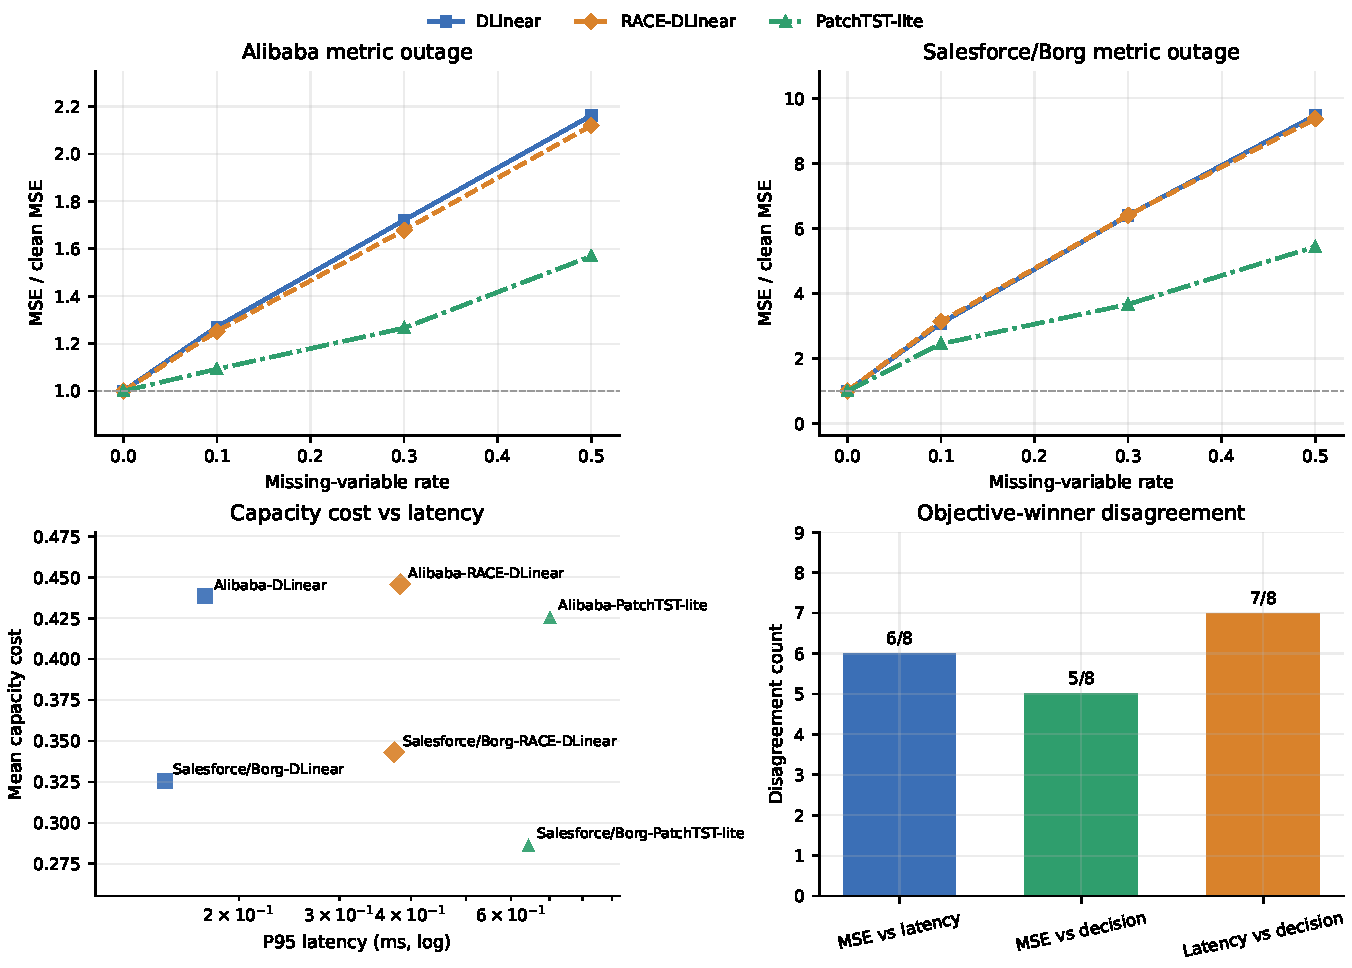
\includegraphics[width=\linewidth]{figure_multisource_deployment_stress.pdf}%
}{%
\fbox{\parbox{0.92\linewidth}{Multi-source deployment-stress figure will be inserted after table and figure generation.}}%
}
\caption{Telemetry degradation changes model-selection tradeoffs across both multivariate sources. Panels show (a) Alibaba metric outage, (b) Salesforce/Borg metric outage, (c) decision cost versus latency, and (d) objective-winner disagreement counts over the same eight compact rows in Table~\ref{tab:cross-source-winners}. The figure supports within-protocol model-selection analysis under controlled offline stress.}
\label{fig:multisource-stress}
\end{figure*}

To reduce the chance that model ranking is an artifact of one random seed, we also run Alibaba and Salesforce/Borg core scenarios with five seeds. Table~\ref{tab:multiseed-compact} reports all 10 core source-stress settings for the lightweight pool. The table separates non-trivial MSE-vs-decision-cost reversals from structural accuracy-vs-latency differences. In the core lightweight pool, MSE and decision-cost winners differ in 4/10 source-stress settings; paired tests over decision cost give $p<0.01$ for all four flips. Separately, DLinear remains the low-latency learned model in all 10 settings.

\begin{table}[t]
\centering
\tiny
\caption{Five-seed winner stability over all 10 core source-stress settings in the lightweight pool. Rows compare the best-MSE, best decision-cost, and lowest-P95 learned models; p-values are paired tests over decision cost for MSE-vs-decision flips.}
\label{tab:multiseed-compact}
\resizebox{\columnwidth}{!}{%
\begin{tabular}{llrllllc}
\toprule
Source & Stress & Seeds & Best MSE & Best decision & Low P95 & MSE != decision & p-value \\
\midrule
Alibaba & Clean & 5 & RACE-DLinear & RACE-DLinear & DLinear & N & -- \\
Alibaba & Delayed tail & 5 & RACE-DLinear & RACE-DLinear & DLinear & N & -- \\
Alibaba & Level shift & 5 & RACE-DLinear & RACE-DLinear & DLinear & N & -- \\
Alibaba & Missing points & 5 & RACE-DLinear & PatchTST-lite & DLinear & Y & 0.0011 \\
Alibaba & Metric outage & 5 & PatchTST-lite & PatchTST-lite & DLinear & N & -- \\
Salesforce/Borg & Clean & 5 & DLinear & RACE-DLinear & DLinear & Y & 0.0007 \\
Salesforce/Borg & Delayed tail & 5 & DLinear & RACE-DLinear & DLinear & Y & 0.0037 \\
Salesforce/Borg & Level shift & 5 & DLinear & RACE-DLinear & DLinear & Y & 0.0064 \\
Salesforce/Borg & Missing points & 5 & PatchTST-lite & PatchTST-lite & DLinear & N & -- \\
Salesforce/Borg & Metric outage & 5 & PatchTST-lite & PatchTST-lite & DLinear & N & -- \\
\bottomrule
\end{tabular}
}
\end{table}


\subsection{Baseline Scope}

Takeaway: the lightweight robust baseline is useful for stress analysis, but the paper's contribution is the benchmark and deployment evidence chain, not a new forecasting architecture.

The ablation explains why RACE-DLinear is not positioned as the main contribution. Removing stress augmentation causes a large degradation on GAIA missing-30, indicating that exposure to deployment-style corruption is more important than the extra model wrapper itself. Masking and calibration affect MAE and capacity cost, but the differences are not stable enough to justify a method-first paper.

This supports the final positioning of the work: the contribution is the controlled stress-to-decision evaluation pipeline and the resulting accuracy--robustness--latency analysis. RACE-DLinear is useful because it tests whether a low-cost robust variant can close part of the gap, but the paper should not claim a universal new forecasting architecture.

\section{Case Studies}

Case-study windows are illustrative and are not used to estimate aggregate performance. The selected cases cover four mechanisms that explain why the aggregate tables matter: NetMan telemetry outage removes the only observable KPI channel, Salesforce/Borg delayed telemetry turns forecasting into stale-context extrapolation, NetMan point missingness exposes an accuracy-latency tradeoff, and Alibaba metric outage stresses cross-metric context. In each case, the clean window hides the degradation mechanism; the aggregate conclusions still come from Tables~\ref{tab:cross-source-winners}--\ref{tab:capacity-sensitivity-compact} and Figure~\ref{fig:multisource-stress}.

\section{Threats to Validity}

\noindent\textbf{Data realism.}
Capacity-related conclusions in this paper are limited to resource-level operational telemetry and should not be extrapolated to service-level SLO behavior. Alibaba 2018 and Salesforce/Borg provide public multivariate operational telemetry, but neither should be over-claimed as a full service-level request/SLO trace. Alibaba is machine-level resource telemetry, and the current Salesforce/Borg subset contains one all-zero dynamic metric. GAIA and NetMan are useful for KPI stress diversity and failure analysis, but they should not be used to make strong resource-capacity claims. A stronger future extension should add a public service-level request, SLO, or autoscaling trace if one becomes reproducibly available.

\noindent\textbf{Forecast-to-capacity decision proxy.}
The forecast-to-capacity evaluator is a reproducible decision proxy, not an autoscaling system. It captures under-provision area, over-provision area, peak misses, and headroom sensitivity, but it does not model queueing, scheduler constraints, cold starts, closed-loop scaling delay, service dependencies, or service-level SLOs. Reactive HPA results therefore cannot be extrapolated to real control conclusions. We use the proxy only for within-protocol comparisons of forecasting-policy consequences.

\noindent\textbf{Baseline fairness.}
Official PatchTST, native iTransformer, and official TimeMixer are integrated into the native stress pipeline for Alibaba and Salesforce/Borg core scenarios. Chronos-Bolt is included only as a bounded zero-shot reference over a subset of windows and should not be read as a complete foundation-model comparison. TimesFM, Moirai, fine-tuned foundation-model variants, and probabilistic FM-specific evaluations are outside the current benchmark scope. Older LTSF CSV bridge runs are retained as reference-only analysis; the bridge flattens entity-metric channels and is not perfectly equivalent to the native per-entity target protocol, so it should not be used as the central ranking claim.

\noindent\textbf{Scope of model claims.}
RACE-DLinear is a lightweight robust baseline, not the main contribution and not a claimed new architecture. The paper's contribution is the benchmark protocol, model-selection analysis, deployment-cost evaluation, and case-study evidence.

\section{Reproducibility and Artifact}

\noindent\textbf{Artifact:} Anonymous review URL to be inserted before submission. The repository contains data conversion scripts, NPZ manifests, stress operators, model wrappers, table-generation scripts, figure-generation scripts, and commands to reproduce Tables~IV--XII and Figure~2.

The anonymous artifact entry point is \texttt{ANON\_ARTIFACT.md}. It includes a benchmark manifest, data conversion scripts, experiment notes, table/figure-generation scripts, and LaTeX sources; repository and license metadata can be finalized for public release after acceptance. Each main table is generated from \texttt{outputs/paper\_tables}, each main figure has a source artifact under \texttt{outputs/paper\_figures}, and the manifest records dataset roles, stress definitions, splits, metrics, and non-claims.

The minimal reproducible path uses the released public NPZ tensors, input length 96, prediction horizon 24, chronological 65/15/20 splits, and seed 42. Running the minimal path regenerates the core clean/stress winner table and the latency summary used in the main paper. Extended runs add severity curves, multi-seed checks, capacity sensitivity, official PatchTST, native iTransformer/TimeMixer, and the bounded Chronos-Bolt reference. We separate the artifact into a minimal reviewer-verification path and an extended evidence path so that the main claims are auditable without requiring reviewers to rerun the full experimental sweep.

\section{Conclusion}

This paper introduced AIOpsStressBench, a reproducible offline stress-to-decision benchmark for operational time-series forecasting. The benchmark combines public telemetry, controlled telemetry-stress operators, latency and memory profiling, severity analysis, and a forecast-to-capacity decision proxy. Under this controlled protocol, clean-MSE selection can differ from the model selected under telemetry degradation, latency budgets, or asymmetric decision costs. This does not imply that clean forecasting benchmarks are uninformative; rather, it shows that they are incomplete for AIOps-style settings where telemetry health and deployment constraints are part of the model-selection problem. Robustness is also stress-family specific: patch-based context can help under metric outage, but this advantage is not universal across noise, delay, and latency-constrained settings. AIOpsStressBench is intended as a complementary evaluation layer for operational forecasting. It is not an autoscaling system, a complete foundation-model benchmark, or a new forecasting architecture claim. Future extensions should add public service-level traces and closed-loop control simulation.

\bibliographystyle{IEEEtran}
\begin{thebibliography}{99}

\bibitem{patchtst}
Y. Nie, N. H. Nguyen, P. Sinthong, and J. Kalagnanam, ``A time series is worth 64 words: Long-term forecasting with transformers,'' in \emph{ICLR}, 2023.

\bibitem{itransformer}
Y. Liu et al., ``iTransformer: Inverted transformers are effective for time series forecasting,'' in \emph{ICLR}, 2024.

\bibitem{dlinear}
A. Zeng, M. Chen, L. Zhang, and Q. Xu, ``Are transformers effective for time series forecasting?'' in \emph{AAAI}, 2023.

\bibitem{timesnet}
H. Wu, T. Hu, Y. Liu, H. Zhou, J. Wang, and M. Long, ``TimesNet: Temporal 2D-variation modeling for general time series analysis,'' in \emph{ICLR}, 2023.

\bibitem{m4}
S. Makridakis, E. Spiliotis, and V. Assimakopoulos, ``The M4 competition: 100,000 time series and 61 forecasting methods,'' \emph{International Journal of Forecasting}, vol. 36, no. 1, pp. 54--74, 2020.

\bibitem{monash}
R. Godahewa, C. Bergmeir, G. I. Webb, R. J. Hyndman, and P. Montero-Manso, ``Monash time series forecasting archive,'' in \emph{NeurIPS Datasets and Benchmarks}, 2021.

\bibitem{gifteval}
T. Aksu, G. Woo, J. Liu, X. Liu, C. Liu, S. Savarese, C. Xiong, and D. Sahoo, ``GIFT-Eval: A benchmark for general time series forecasting model evaluation,'' arXiv:2410.10393, 2024.

\bibitem{fevbench}
O. Shchur, A. F. Ansari, C. Turkmen, L. Stella, N. Erickson, P. Guerron, M. Bohlke-Schneider, and Y. Wang, ``fev-bench: A realistic benchmark for time series forecasting,'' arXiv:2509.26468, 2025.

\bibitem{alibaba}
Alibaba Cluster Trace Program, ``Alibaba cluster trace 2018,'' 2018.

\bibitem{timemixer}
S. Wang, H. Wu, X. Shi, T. Hu, H. Luo, L. Ma, J. Zhang, and J. Zhou, ``TimeMixer: Decomposable multiscale mixing for time series forecasting,'' in \emph{ICLR}, 2024.

\bibitem{chronos}
A. F. Ansari et al., ``Chronos: Learning the language of time series,'' \emph{Transactions on Machine Learning Research}, 2024.

\bibitem{moirai}
G. Woo, C. Liu, A. Kumar, C. Xiong, S. Savarese, and D. Sahoo, ``Unified training of universal time series forecasting transformers,'' in \emph{ICML}, 2024.

\bibitem{timesfm}
A. Das, W. Kong, R. Sen, and Y. Zhou, ``A decoder-only foundation model for time-series forecasting,'' arXiv:2310.10688, 2023.

\bibitem{fmenergy}
L. Guibert, B. Pasquier, F. Montet, and B. Wolf, ``Benchmarking time series foundation models on their accuracy and energy consumption,'' in \emph{Proceedings of the Swiss AI Days}, PMLR 309, 2026.

\bibitem{cloudops}
G. Woo, C. Liu, A. Kumar, and D. Sahoo, ``Pushing the limits of pre-training for time series forecasting in the CloudOps domain,'' arXiv:2310.05063, 2023.

\bibitem{boom}
B. Cohen et al., ``This time is different: An observability perspective on time series foundation models,'' arXiv:2505.14766, 2025.

\bibitem{autopilot}
K. Rzadca et al., ``Autopilot: Workload autoscaling at Google,'' in \emph{EuroSys}, 2020.

\bibitem{sinan}
Y. Zhang, W. Hua, Z. Zhou, G. E. Suh, and C. Delimitrou, ``Sinan: ML-based and QoS-aware resource management for cloud microservices,'' in \emph{ASPLOS}, 2021.

\bibitem{ahpa}
Z. Zhou, C. Zhang, L. Ma, J. Gu, H. Qian, Q. Wen, L. Sun, P. Li, and Z. Tang, ``AHPA: Adaptive horizontal pod autoscaling systems on Alibaba Cloud Container Service for Kubernetes,'' in \emph{AAAI}, 2024.

\bibitem{gcm_missing}
Google Cloud, ``Behavior of metric-based alerting policies: Missing data,'' Cloud Monitoring documentation.

\bibitem{gcm_latency}
Google Cloud, ``Metric latency and data freshness,'' Cloud Monitoring documentation.

\bibitem{prom_staleness}
Prometheus Authors, ``Staleness,'' Prometheus documentation.

\bibitem{k8s_hpa}
Kubernetes Authors, ``Horizontal Pod Autoscaling,'' Kubernetes documentation.

\bibitem{grud}
Z. Che, S. Purushotham, K. Cho, D. Sontag, and Y. Liu, ``Recurrent neural networks for multivariate time series with missing values,'' \emph{Scientific Reports}, vol. 8, 2018.

\bibitem{brits}
W. Cao, D. Wang, J. Li, H. Zhou, L. Li, and Y. Li, ``BRITS: Bidirectional recurrent imputation for time series,'' in \emph{NeurIPS}, 2018.

\bibitem{onenet}
Y.-F. Zhang, Q. Wen, X. Wang, W. Chen, L. Sun, Z. Zhang, L. Wang, R. Jin, and T. Tan, ``OneNet: Enhancing time series forecasting models under concept drift by online ensembling,'' in \emph{NeurIPS}, 2023.

\bibitem{woods}
J.-C. Gagnon-Audet, K. Ahuja, M.-J. Darvishi-Bayazi, P. Mousavi, G. Dumas, and I. Rish, ``WOODS: Benchmarks for out-of-distribution generalization in time series,'' \emph{Transactions on Machine Learning Research}, 2023.

\bibitem{gaia}
CloudWise-OpenSource, ``GAIA-DataSet: Generic AIOps Atlas,'' GitHub repository, 2021.

\bibitem{netman}
Z. Li, N. Zhao, S. Zhang, Y. Sun, P. Chen, X. Wen, M. Ma, and D. Pei, ``Constructing large-scale real-world benchmark datasets for AIOps,'' arXiv:2208.03938, 2022.

\end{thebibliography}

\end{document}
